\subsection{Benchmarking for Employee Use Case}
%- What did we benchmark?
%Explain which scenarios we did test (1 employee, multiple employee)
We especially benchmarked the employee use case as the employee use case is the more complex one of our both use cases. As a preparation for benchmarking we first needed two different smart contracts. One smart contract that works completely on-chain without using any external database, hashing functions or Merkle trees and another smart contract that uses all introduced methods that are needed in order to off-chain our data to an external database. The two variants behave completely similar except for the saving of the state variables. Both variants are completely functional and could be used as they are if someone would like to deploy the employee use case. These fact were very important to us because only like that we could make sure that our benchmarks lead to meaningful results. Within the employee use case we measured different scenarios which will be described in the corresponding sections, mainly a time measure as well as a simple and another complex measure for the gas cost have been made.

%Explain under which aspects we did benchmark (gas, time)
%Mention again why gas is of utmost importance to us (because it translates to money and time)
%Explain the thing with benchmarking only the overhead due to automining of ganache
We mainly benchmarked the two measurements gas cost and time. Gas cost was the initial motivation for off-chaining as we assumed to save on gas cost when we off-chain the state variables. Gas cost translates to real currency as a participant of the blockchain either needs to buy Ether or help to mine blocks in order to receive Ether which is needed to pay the resulting gas cost of a transaction. The time was measured as we wanted to gain insights into how much overhead our application adds to a normal blockchain application. This was possible as our technology stack includes ganache which is capable of automatically mining new transactions into new blocks instantly so that we are able to measure only the overhead that our application introduces.

%- Nice transition into showing our first graphics.
\subsubsection{Time measurement}
First we will measure the introduced computation time of our application for executing different functions of the smart contract. The result can be seen in Figure \ref{fig:05_time}.

\begin{figure}[t]%evtl:[t] [!htbp]
\centering
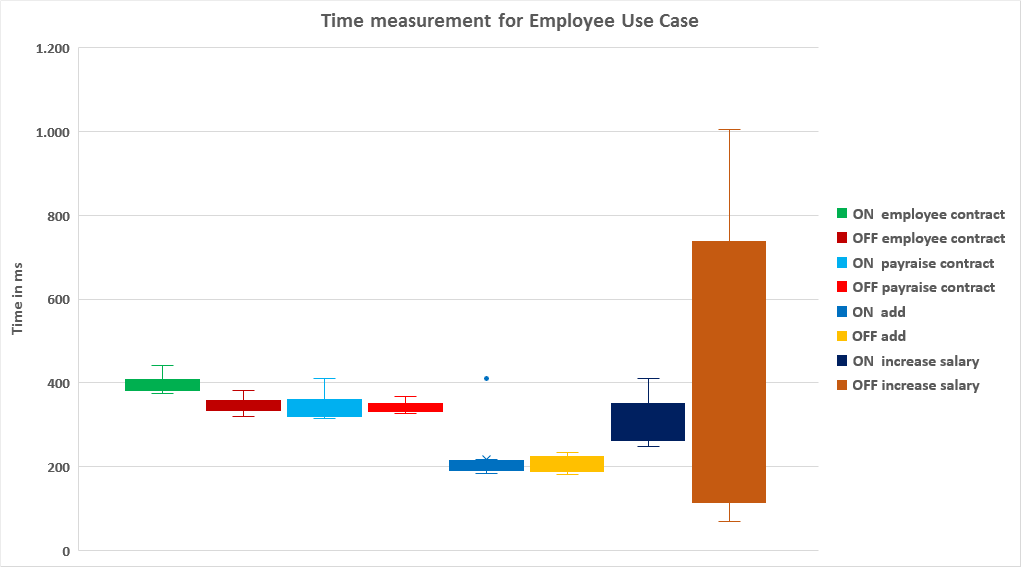
\includegraphics[width=1.0\textwidth]{images/05_evaluation/05_time.png}
\caption{\label{fig:05_time}Time measurement for Employee Use Case.}
\end{figure}

%Thats a box plot chart
As we measured the computation time multiple times we decided to unite the results into a box plot chart. Thus we can see how the system behaves most of the times and single outliers can easily be identified. Throughout our measurement we always compare the on-chained approach against the off-chained approach. Every single function got called multiple times and the results have been summed up into the corresponding box plot.

For the \textit{employee contract} creation we can see the that the time differs by circa 50ms when comparing the on-chained approach to the off-chained approach. The on-chained approach needs about 400ms of computation time in the application while the off-chained approach needs 350ms. Both timings are negligible for us as the average block time of the Ethereum blockchain is currently about 14 seconds \cite{etherscan_blocktime}. Thus our application has more than enough time to compute a new transaction comparing nearly half a second against 14 seconds.

The \textit{payraise contract} creation needs about the same time for the on-chained as for the off-chained approach. Both need about 350ms of computation time and are negligible for the same reason as for the \textit{employee contract} creation. The same holds true for the \textit{add} functionality which takes even less time and thus the timing is negligible here as well.

More interesting are the timing needs of the \textit{increase salary} functionality. We can easily see that the off-chained variant has a much higher variance than the on-chained variant and we have peeks in the computation time of up to one second. Hereby it is very important to mention that the time needed for the off-chained variant increases with the size of the employee dataset. This happens because for every added employee the \textit{increase salary} function needs to generate another transaction. As every transaction needs to be mined first the increased timing needs of our application are also negligible as what we see in our chart is the cumulated computation time for all transactions that happened during this function call. All of these transactions need to be mined within blocks of the Ethereum blockchain which takes a lot longer, namely about 14 seconds currently, than the computation of our application. Plus, it could possibly happen that the single transactions will be divided on multiple blocks. Therefore the introduced timing needs of our application are also negligible for this function and additionally all measurements of the \textit{increase salary} function were less than a second which is quite fast.% maybe explain that the introduced overhead is somehow "virtual?"

%Everything under 1 second -> not relevant, no further measurements
%Erwähnen dass es super ist, dass die middlewar keine extra zeiten introduced und genauso fix ist wie das normale.
As every function call in the off-chained approach does not introduce a real overhead compared to the on-chained approach and our application always performed under one second we concluded that we do not need to deeper analyze what introduces the most computation time or how to optimize for time in our application as this would not include a great benefit for our use case. Therefore no further measurements concerning the computation time have been made. We can conclude that the off-chained approach did not introduce any additional computation time and is as good as the on-chained approach timewise.

\subsubsection{Gas cost measurement}
Measuring the gas needed for executing the functionalities of our smart contract is of utmost importance to us. The initial motivation for our prototype was to gain experience on whether it is possible to save on gas cost when off-chaining state variables from smart contracts. As we receive the used gas for each transaction within the JSON-response when we call the smart contract functions through our API endpoint we were able to extract different insights into the use of gas when on- or off-chaining.

%And smth more in Figure \ref{fig:05_gas_cost_single}.
In Figure \ref{fig:05_gas_cost_single} we visualized the used gas for calling single functions of our smart contract for the employee use case. Similarly to our time measurement we again measured the main functionalities of our smart contract and compared the on-chained variant with the off-chained variant. The results of our analysis will be discussed now.

\begin{figure}[t]
\centering
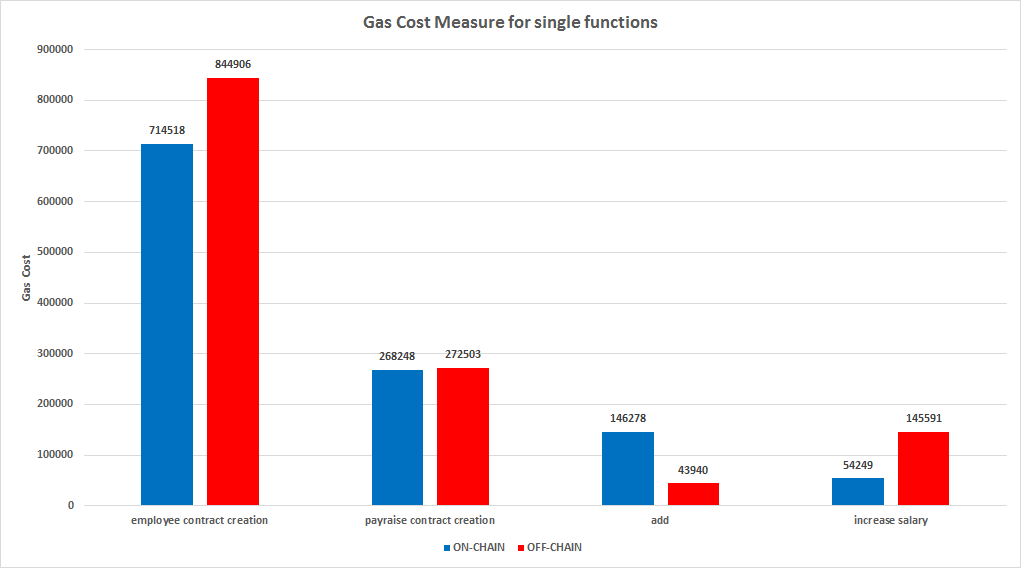
\includegraphics[width=1.0\textwidth]{images/05_evaluation/05_gas_cost_single.png}
\caption{\label{fig:05_gas_cost_single}This is one employee.}
\end{figure}

%- employee creation more costy because overhead of functions for Merkle tree (elaborate what exactly here)
% 844906 - 714518 = 130388 gas,    130388 / 714518 = 18,25%
%    results) in a future work which could be making library identifies future work
% besides from empty lists 
%Say why we save and then in the end say that its constant and how much percentage-wise this translates to
%Blabla could be optimized by making those functions libraries
For the \textit{employee contract} creation we can see that the off-chained variant needs about 130 thousand more gas than the on-chained variant. Both smart contracts do not save any state variables yet apart from empty lists for either hash values or employees, depending on the approach. The difference in the gas cost originates mainly from the added functions for the Merkle tree proof and verification which were added to the smart contract for the off-chained approach. Thanks to this finding a new task for future work could be identified. Extracting the functions which are needed in order to iterate through the tree and verify the Merkle proof into a library in the sense of Solidity would benefit the off-chaining approach. Calling functions of libraries in Solidity is in general very beneficial in terms of gas cost. Anyways the gas cost of the off-chained approach exceed the gas cost of the on-chained approach only by approximately 18\% which is rather minor. All in all, it can be said that the increased gas cost of the off-chained approach are negligible as the contract creation needs to be paid only once throughout the whole life cycle of the smart contract. Analyzing the offered functions of the smart contract is much more important as these will be called multiple times.

%- payraise not changed (on-chained for both, thats why it is the same)
The gas cost for the creation of the \textit{payraise contract} do not differ from each other as both approaches use the same implementation for the payraise contract. The payraise contract holds very few information in his state variables which basically are information about the department for the payraise and a percentage value for the payraise. Off-Chaining this very small contract would not have made sense and thus it was kept as an on-chain approach because this contract is not very data intense.

% - on add we save xy gas because thats where off-chaining is stronk
% independent of data we always pay 43940, even if employee bigger or more fields blabla whatever, this is super constant which is huge
% 146278 - 43940 = 102388,      43490 / 146278 = 30, 04% --> We save 70%
% Comparing this to constant overhead is enormous because we save what we lost with only one call
One of the most interesting functions of the smart contract is the \textit{add} functionality. This is one of the main features of the employee contract which we expected to yield the biggest opportunity to save on gas cost. Our measurements confirmed our expectations as we save approximately 102 thousand gas on each call of the \textit{add} functionality which translates to a save of about 70\%. An important thing to mention at this point is that the gas cost of 43940 for the off-chained \textit{add} functionality are constant because that is the gas cost for saving one root hash in a smart contract. So independent of how big the employee data item looks like, so independent whether it uses very long or short names, we will always only need to pay the constant 43940 gas for storing the hash of this record. This would also hold true if there were multiple new variable fields added to employee records in general. Comparing the savings of the \textit{add} functionality to the introduced overhead when saving employee contracts where we needed to pay about 130 thousand gas more lets the overhead look very small because by adding only one employee we nearly balanced this overhead out. Bigger savings could be achieved by adding multiple employees which represents a normal use case.

% 145591 - 54249 = 91342,   145591 / 54249 = 268,38% :'(
%- increase salary we loose because [.....] only one field, multiple transactions, elaborate on possible alternatives like functions that would change multiple strings etc etc
Another very important function is the \textit{increase salary} functionality of the employee contract. We can see that the gas cost for increasing the salary of a single employee raises by approximately 91 thousand gas for the off-chained approach. This happens because in the case of increasing salary only one integer field of an employee gets changed which is a very small variable type. The on-chained variant only needs to iterate through its locally saved employees and increase the salary for a given employee, in our case the list would only contain one employee. Increasing the salary translates to saving a new integer variable as a state variable of the smart contract which is compared to the off-chained approach rather cheap in terms of gas cost. The off-chained approach however sends the integer field for the salary of the employee together with a complete Merkle proof for verifying the integrity of this salary field. The smart contract would then need to start his computations by verifying the integrity of the received employee respectively the salary of the employee. The overhead introduced by this behavior explains the risen gas cost for the off-chained approach.

Introducing more functionalities would make the evaluation even more complex. One could think of a new function that would modify multiple string fields of the employee which would lead to the need of paying for the newly saved string fields. In such a similarly constructed function like the \textit{increase salary} functionality the off-chained approach would not perform worse than the on-chained approach. The on-chained approach would have to pay high gas costs for the saving of multiple string variables into its state while the off-chained approach would only have the same overhead of the sent Merkle proof and verification.

%Blabla Use case dependent, therefore further measurements oder too simple therefore a more complex scenario
%And yet smth more in Figure \ref{fig:05_gas_cost_ten}.
As we identified that there exist circumstances in which the off-chained approach performs better and circumstances in which the state of the art on-chained approach performs better we decided to benchmark a more complex scenario of the employee use case. As the gas cost for the creation of the contracts are constant we decided to focus on the functionalities which can be called multiple times and can have varying results. We introduce a scenario where we add 10 different employees with varying data which are divided up into two different departments. 8 of those employees work in the 'IT' department while the other 2 employees work in the 'Marketing and Management' department. This was introduced so we can benchmark how the \textit{increase salary} function behaves when it gets executed on the majority of the employees or respectively on the minority. The results for the cumulative gas costs of this benchmark are visualized in Figure \ref{fig:05_gas_cost_ten}.

\begin{figure}[t]%[htbp]
\centering
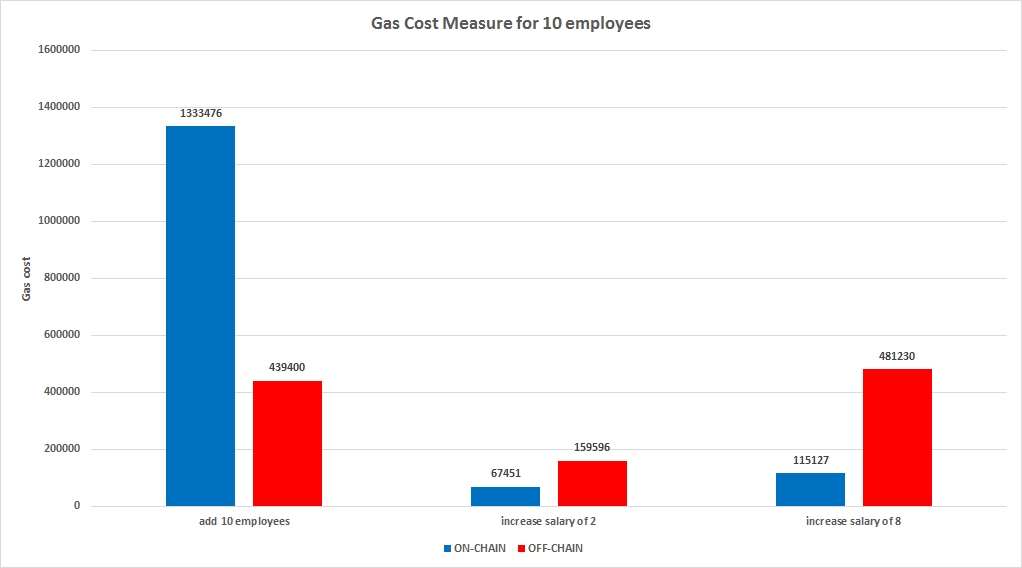
\includegraphics[width=1.0\textwidth]{images/05_evaluation/05_gas_cost_ten.png}
\caption{\label{fig:05_gas_cost_ten}This is ten employees.}
\end{figure}

% 1333476 - 439400 = 894076,   439400 / 1333476 = 32,95% -> 67%
When adding 10 employees to the employee contract we can see that the overall saving on gas was approximately 894 thousand gas. Also we see that the off-chained approach needed exactly 439400 gas which is exactly the tenfold of the constant gas cost for adding a single root hash to the smart contract which aligns with our thoughts on that. The cumulative gas cost for the on-chained approach are put together by slightly differing gas costs for each add call as we used different data for the added employees so the single add values would fluctuate.

% 159596 - 67451 = 92451,   159596 / 67451 = 236,61% -> 237%
% 481230 - 115127 = 366103,   481230 / 115127 = 418%
Most interesting for us is the finding that the \textit{increase salary} function behaves differently when calling it on the majority or respectively on the minority of the employees. If we look at the percentage-wise increase of the gas cost for the off-chained variant a huge difference gets visible.
$$ 159596 / 67451 \approx 237\% $$
$$ 481230 / 115127 \approx 418\% $$
Here we can clearly see that when we update the majority of the employees the overhead of the off-chained variant becomes greater. This has mainly two reasons. The first reason lays in the behavior of the on-chained approach because when calling the \textit{increase salary} function it iterates over all saved employees in order to find the employees of the requested department. This iterating is more costy when only few of the employees get matched so the on-chained approach is weaker in terms of performance when updating the minority. The second reason lays in the behavior of the off-chained approach. The off-chained approach can easily query the departments in the RDBMS without using blockchain computation power and afterwards send only the needed employees to the smart contract and thus save when updating the minority. On the other hand with every sent employee the overhead for the Merkle proof and verification gets added as well as the cost for creating a transaction to the blockchain which leads to a bigger increase when updating the majority of the employees.

%- Know your use case!
%Do we really save gas?
%mention all or nothing approach (can be either off-chained completely or on-chained completely)
As mentioned before there are functions in which the off-chained approach performs better and other functions where it is less efficient. The most important thing when deciding whether to off-chain an existing contract is to know the use case very well, especially the ratio of how often the functions are called compared to each other. In our use case we can assume that employees will get added more often than the salary will be increased, this is why off-chaining makes sense here. Also it is important to mention that when off-chaining there is no possibility to decide whether to off-chain the add method but keep the \textit{increase salary} function on-chain because each approach needs the data at a certain place. So either all functions get off-chained or none. Thus one has to carefully decide whether the savings on the one side will outweigh the overhead on the other side. There are plenty of use cases for which this is true.

%When does Off-Chaining make sense?
%- Give pay-raise as example for when off-chaining makes no sense (we kept it on-chain)
In general we can say that off-chaining makes especially sense when smart contracts use mainly big state variables and functions which change big or many variables of the state of the smart contract. For smaller contracts which do not save a lot of variables or are rather of a computational intense nature off-chaining does not make sense as it would introduce an unnecessary overhead. We can see an example for that in the payraise contract. As this contract was so small we did not off-chain it as this would have introduced a bigger overhead due to the Merkle proof and verification.

%- Later on say how our measurements can be compared to the financials use case (cut out the increase-salary basically)
Comparing the measurements for the employee use case to the financial use case we can say that the results would probably have been very similar as the financials use case has similar structure compared to the employee use case. In the financials use case we save a lot of financials data so we would probably also save on the \textit{add} functionality but the verification of the financial records would be conducted offline and not on the blockchain. This is why an evaluation for the financials use case would look very similar to the evaluation of the employee use case with the main difference of not gaining the insights we gained when analyzing the \textit{increase salary} function as the financials use case has no equivalent for this function.

%- Elaborate on conclusions and findings from this evaluation
%-> Conclude on that
